\documentclass[twoside]{book}

% Packages required by doxygen
\usepackage{fixltx2e}
\usepackage{calc}
\usepackage{doxygen}
\usepackage[export]{adjustbox} % also loads graphicx
\usepackage{graphicx}
\usepackage[utf8]{inputenc}
\usepackage{makeidx}
\usepackage{multicol}
\usepackage{multirow}
\PassOptionsToPackage{warn}{textcomp}
\usepackage{textcomp}
\usepackage[nointegrals]{wasysym}
\usepackage[table]{xcolor}

% Font selection
\usepackage[T1]{fontenc}
\usepackage[scaled=.90]{helvet}
\usepackage{courier}
\usepackage{amssymb}
\usepackage{sectsty}
\renewcommand{\familydefault}{\sfdefault}
\allsectionsfont{%
  \fontseries{bc}\selectfont%
  \color{darkgray}%
}
\renewcommand{\DoxyLabelFont}{%
  \fontseries{bc}\selectfont%
  \color{darkgray}%
}
\newcommand{\+}{\discretionary{\mbox{\scriptsize$\hookleftarrow$}}{}{}}

% Page & text layout
\usepackage{geometry}
\geometry{%
  a4paper,%
  top=2.5cm,%
  bottom=2.5cm,%
  left=2.5cm,%
  right=2.5cm%
}
\tolerance=750
\hfuzz=15pt
\hbadness=750
\setlength{\emergencystretch}{15pt}
\setlength{\parindent}{0cm}
\setlength{\parskip}{3ex plus 2ex minus 2ex}
\makeatletter
\renewcommand{\paragraph}{%
  \@startsection{paragraph}{4}{0ex}{-1.0ex}{1.0ex}{%
    \normalfont\normalsize\bfseries\SS@parafont%
  }%
}
\renewcommand{\subparagraph}{%
  \@startsection{subparagraph}{5}{0ex}{-1.0ex}{1.0ex}{%
    \normalfont\normalsize\bfseries\SS@subparafont%
  }%
}
\makeatother

% Headers & footers
\usepackage{fancyhdr}
\pagestyle{fancyplain}
\fancyhead[LE]{\fancyplain{}{\bfseries\thepage}}
\fancyhead[CE]{\fancyplain{}{}}
\fancyhead[RE]{\fancyplain{}{\bfseries\leftmark}}
\fancyhead[LO]{\fancyplain{}{\bfseries\rightmark}}
\fancyhead[CO]{\fancyplain{}{}}
\fancyhead[RO]{\fancyplain{}{\bfseries\thepage}}
\fancyfoot[LE]{\fancyplain{}{}}
\fancyfoot[CE]{\fancyplain{}{}}
\fancyfoot[RE]{\fancyplain{}{\bfseries\scriptsize Generated by Doxygen }}
\fancyfoot[LO]{\fancyplain{}{\bfseries\scriptsize Generated by Doxygen }}
\fancyfoot[CO]{\fancyplain{}{}}
\fancyfoot[RO]{\fancyplain{}{}}
\renewcommand{\footrulewidth}{0.4pt}
\renewcommand{\chaptermark}[1]{%
  \markboth{#1}{}%
}
\renewcommand{\sectionmark}[1]{%
  \markright{\thesection\ #1}%
}

% Indices & bibliography
\usepackage{natbib}
\usepackage[titles]{tocloft}
\setcounter{tocdepth}{3}
\setcounter{secnumdepth}{5}
\makeindex

% Hyperlinks (required, but should be loaded last)
\usepackage{ifpdf}
\ifpdf
  \usepackage[pdftex,pagebackref=true]{hyperref}
\else
  \usepackage[ps2pdf,pagebackref=true]{hyperref}
\fi
\hypersetup{%
  colorlinks=true,%
  linkcolor=blue,%
  citecolor=blue,%
  unicode%
}

% Custom commands
\newcommand{\clearemptydoublepage}{%
  \newpage{\pagestyle{empty}\cleardoublepage}%
}

\usepackage{caption}
\captionsetup{labelsep=space,justification=centering,font={bf},singlelinecheck=off,skip=4pt,position=top}

%===== C O N T E N T S =====

\begin{document}

% Titlepage & ToC
\hypersetup{pageanchor=false,
             bookmarksnumbered=true,
             pdfencoding=unicode
            }
\pagenumbering{alph}
\begin{titlepage}
\vspace*{7cm}
\begin{center}%
{\Large tetris \\[1ex]\large final beta }\\
\vspace*{1cm}
{\large Generated by Doxygen 1.8.13}\\
\end{center}
\end{titlepage}
\clearemptydoublepage
\pagenumbering{roman}
\tableofcontents
\clearemptydoublepage
\pagenumbering{arabic}
\hypersetup{pageanchor=true}

%--- Begin generated contents ---
\chapter{R\+E\+A\+D\+ME}
\label{md_README}
\Hypertarget{md_README}
Hello!

This project is simple implementation of the Tetris famous game. I\textquotesingle{}ve made it mainly for learning purpose. I don\textquotesingle{}t think that you will find pleasure playing with it, but if you are developer, you can read the source code which is documented. Hope that it\textquotesingle{}ll allow you to learn things.

To install this program on Linux, first download it\+: 
\begin{DoxyCode}
git clone https://github.com/authmane512/tetris.git
cd tetris
\end{DoxyCode}


Before compile it, you need S\+D\+L2 library which you can install like that on Debian\+: 
\begin{DoxyCode}
sudo apt install libsdl2-dev
\end{DoxyCode}


Then you can compile the code\+: 
\begin{DoxyCode}
make
\end{DoxyCode}


Finally start the program\+: 
\begin{DoxyCode}
./tetris
\end{DoxyCode}
 
\chapter{Class Index}
\section{Class List}
Here are the classes, structs, unions and interfaces with brief descriptions\+:\begin{DoxyCompactList}
\item\contentsline{section}{\hyperlink{structttm}{ttm} \\*Structure for tetriminos }{\pageref{structttm}}{}
\end{DoxyCompactList}

\chapter{File Index}
\section{File List}
Here is a list of all documented files with brief descriptions\+:\begin{DoxyCompactList}
\item\contentsline{section}{\hyperlink{debugging_8c}{debugging.\+c} \\*Lot of functions for debugging purpose }{\pageref{debugging_8c}}{}
\item\contentsline{section}{{\bfseries debugging.\+h} }{\pageref{debugging_8h}}{}
\item\contentsline{section}{{\bfseries events.\+h} }{\pageref{events_8h}}{}
\item\contentsline{section}{{\bfseries load\+\_\+graphics.\+h} }{\pageref{load__graphics_8h}}{}
\item\contentsline{section}{\hyperlink{main_8c}{main.\+c} \\*Main part of the code }{\pageref{main_8c}}{}
\item\contentsline{section}{{\bfseries main.\+h} }{\pageref{main_8h}}{}
\item\contentsline{section}{{\bfseries sdl.\+h} }{\pageref{sdl_8h}}{}
\item\contentsline{section}{platforms/android/{\bfseries events.\+h} }{\pageref{platforms_2android_2events_8h}}{}
\item\contentsline{section}{platforms/android/{\bfseries load\+\_\+graphics.\+h} }{\pageref{platforms_2android_2load__graphics_8h}}{}
\item\contentsline{section}{platforms/desktop/\hyperlink{desktop_2events_8c}{events.\+c} }{\pageref{desktop_2events_8c}}{}
\item\contentsline{section}{platforms/desktop/{\bfseries events.\+h} }{\pageref{platforms_2desktop_2events_8h}}{}
\item\contentsline{section}{platforms/desktop/\hyperlink{desktop_2load__graphics_8c}{load\+\_\+graphics.\+c} }{\pageref{desktop_2load__graphics_8c}}{}
\item\contentsline{section}{platforms/desktop/{\bfseries load\+\_\+graphics.\+h} }{\pageref{platforms_2desktop_2load__graphics_8h}}{}
\end{DoxyCompactList}

\chapter{Class Documentation}
\hypertarget{structttm}{}\section{ttm Struct Reference}
\label{structttm}\index{ttm@{ttm}}


structure for tetriminos  


\subsection*{Public Attributes}
\begin{DoxyCompactItemize}
\item 
char \hyperlink{structttm_ae996fb75cf767777192617821fb94191}{mat} \mbox{[}T\+T\+M\+\_\+\+W\+I\+D\+TH\mbox{]}\mbox{[}T\+T\+M\+\_\+\+W\+I\+D\+TH\mbox{]}
\item 
int \hyperlink{structttm_ad31396b959fc09891926ea70dac0a985}{row}
\item 
int \hyperlink{structttm_a5803d7706ed98e36ccd7c78568ac3c58}{col}
\item 
int \hyperlink{structttm_a576f3b3a777fd0b70e06e8a988fbce00}{printed}
\end{DoxyCompactItemize}


\subsection{Detailed Description}
structure for tetriminos 

\subsection{Member Data Documentation}
\mbox{\Hypertarget{structttm_a5803d7706ed98e36ccd7c78568ac3c58}\label{structttm_a5803d7706ed98e36ccd7c78568ac3c58}} 
\index{ttm@{ttm}!col@{col}}
\index{col@{col}!ttm@{ttm}}
\subsubsection{\texorpdfstring{col}{col}}
{\footnotesize\ttfamily ttm\+::col}

The column of the tetrimino in the board \mbox{\Hypertarget{structttm_ae996fb75cf767777192617821fb94191}\label{structttm_ae996fb75cf767777192617821fb94191}} 
\index{ttm@{ttm}!mat@{mat}}
\index{mat@{mat}!ttm@{ttm}}
\subsubsection{\texorpdfstring{mat}{mat}}
{\footnotesize\ttfamily ttm\+::mat}

The matrix of the tetrimino \mbox{\Hypertarget{structttm_a576f3b3a777fd0b70e06e8a988fbce00}\label{structttm_a576f3b3a777fd0b70e06e8a988fbce00}} 
\index{ttm@{ttm}!printed@{printed}}
\index{printed@{printed}!ttm@{ttm}}
\subsubsection{\texorpdfstring{printed}{printed}}
{\footnotesize\ttfamily ttm\+::printed}

Equal to 1 if the tetrimino is full down and can no more be moved \mbox{\Hypertarget{structttm_ad31396b959fc09891926ea70dac0a985}\label{structttm_ad31396b959fc09891926ea70dac0a985}} 
\index{ttm@{ttm}!row@{row}}
\index{row@{row}!ttm@{ttm}}
\subsubsection{\texorpdfstring{row}{row}}
{\footnotesize\ttfamily ttm\+::row}

The row of the tetrimino in the board 

The documentation for this struct was generated from the following file\+:\begin{DoxyCompactItemize}
\item 
\hyperlink{main_8c}{main.\+c}\end{DoxyCompactItemize}

\chapter{File Documentation}
\hypertarget{debugging_8c}{}\section{debugging.\+c File Reference}
\label{debugging_8c}\index{debugging.\+c@{debugging.\+c}}


a lot of functions for debugging purpose  


{\ttfamily \#include $<$stdio.\+h$>$}\newline
{\ttfamily \#include $<$stdlib.\+h$>$}\newline
{\ttfamily \#include $<$string.\+h$>$}\newline
{\ttfamily \#include \char`\"{}debugging.\+h\char`\"{}}\newline
Include dependency graph for debugging.\+c\+:
\nopagebreak
\begin{figure}[H]
\begin{center}
\leavevmode
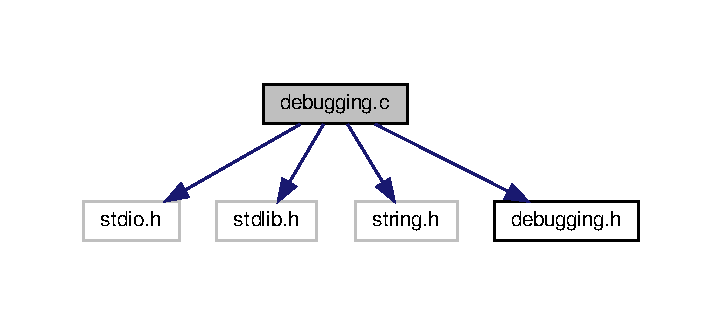
\includegraphics[width=347pt]{debugging_8c__incl}
\end{center}
\end{figure}
\subsection*{Functions}
\begin{DoxyCompactItemize}
\item 
\mbox{\Hypertarget{debugging_8c_af0741d8fa875bd5a94bdf4e288521910}\label{debugging_8c_af0741d8fa875bd5a94bdf4e288521910}} 
long {\bfseries min} (int $\ast$arr, long len)
\item 
\mbox{\Hypertarget{debugging_8c_aeb832e48b81348434bbdc67b0d4f6d1c}\label{debugging_8c_aeb832e48b81348434bbdc67b0d4f6d1c}} 
long {\bfseries max} (int $\ast$arr, long len)
\item 
\mbox{\Hypertarget{debugging_8c_a23af56c60294db34e82ee1cef3e2f452}\label{debugging_8c_a23af56c60294db34e82ee1cef3e2f452}} 
long {\bfseries sum} (int $\ast$arr, long len)
\item 
\mbox{\Hypertarget{debugging_8c_a27937d17b015f556b737d55e2477d0ba}\label{debugging_8c_a27937d17b015f556b737d55e2477d0ba}} 
void {\bfseries rotate} (int $\ast$$\ast$matrix, long rows, long cols)
\item 
\mbox{\Hypertarget{debugging_8c_a6bfbccbe1016f63095ae0e54e07bf619}\label{debugging_8c_a6bfbccbe1016f63095ae0e54e07bf619}} 
void {\bfseries print\+Arr} (int $\ast$arr, long len)
\item 
\mbox{\Hypertarget{debugging_8c_a748793db3cc346bdaad5a9bf257ac53d}\label{debugging_8c_a748793db3cc346bdaad5a9bf257ac53d}} 
void {\bfseries print\+Matrix} (int $\ast$$\ast$matrix, long rows, long cols)
\item 
\mbox{\Hypertarget{debugging_8c_a4583bcc9bde28713555615d595dbec72}\label{debugging_8c_a4583bcc9bde28713555615d595dbec72}} 
long {\bfseries read\+Arr} (int $\ast$arr)
\item 
\mbox{\Hypertarget{debugging_8c_a2b041d219c693911005f8276b8dcb29d}\label{debugging_8c_a2b041d219c693911005f8276b8dcb29d}} 
int {\bfseries cmp} (const void $\ast$x, const void $\ast$y)
\item 
\mbox{\Hypertarget{debugging_8c_a1acffac288acf6e0b8947b6457fffff2}\label{debugging_8c_a1acffac288acf6e0b8947b6457fffff2}} 
int {\bfseries rcmp} (const void $\ast$x, const void $\ast$y)
\item 
\mbox{\Hypertarget{debugging_8c_ace092f3dec388c641a254c03499f8196}\label{debugging_8c_ace092f3dec388c641a254c03499f8196}} 
void {\bfseries sort} (int $\ast$arr, long len, int reverse)
\item 
\mbox{\Hypertarget{debugging_8c_a3a910988a9f842d83dc13eceb18b96a7}\label{debugging_8c_a3a910988a9f842d83dc13eceb18b96a7}} 
void {\bfseries reverse\+Arr} (int $\ast$arr, long len)
\end{DoxyCompactItemize}


\subsection{Detailed Description}
a lot of functions for debugging purpose 


\hypertarget{main_8c}{}\section{main.\+c File Reference}
\label{main_8c}\index{main.\+c@{main.\+c}}


main part of the code  


{\ttfamily \#include $<$time.\+h$>$}\newline
{\ttfamily \#include $<$stdlib.\+h$>$}\newline
{\ttfamily \#include $<$string.\+h$>$}\newline
{\ttfamily \#include $<$stdio.\+h$>$}\newline
{\ttfamily \#include \char`\"{}main.\+h\char`\"{}}\newline
{\ttfamily \#include \char`\"{}sdl.\+h\char`\"{}}\newline
{\ttfamily \#include \char`\"{}debugging.\+h\char`\"{}}\newline
{\ttfamily \#include \char`\"{}events.\+h\char`\"{}}\newline
{\ttfamily \#include \char`\"{}load\+\_\+graphics.\+h\char`\"{}}\newline
Include dependency graph for main.\+c\+:
\nopagebreak
\begin{figure}[H]
\begin{center}
\leavevmode
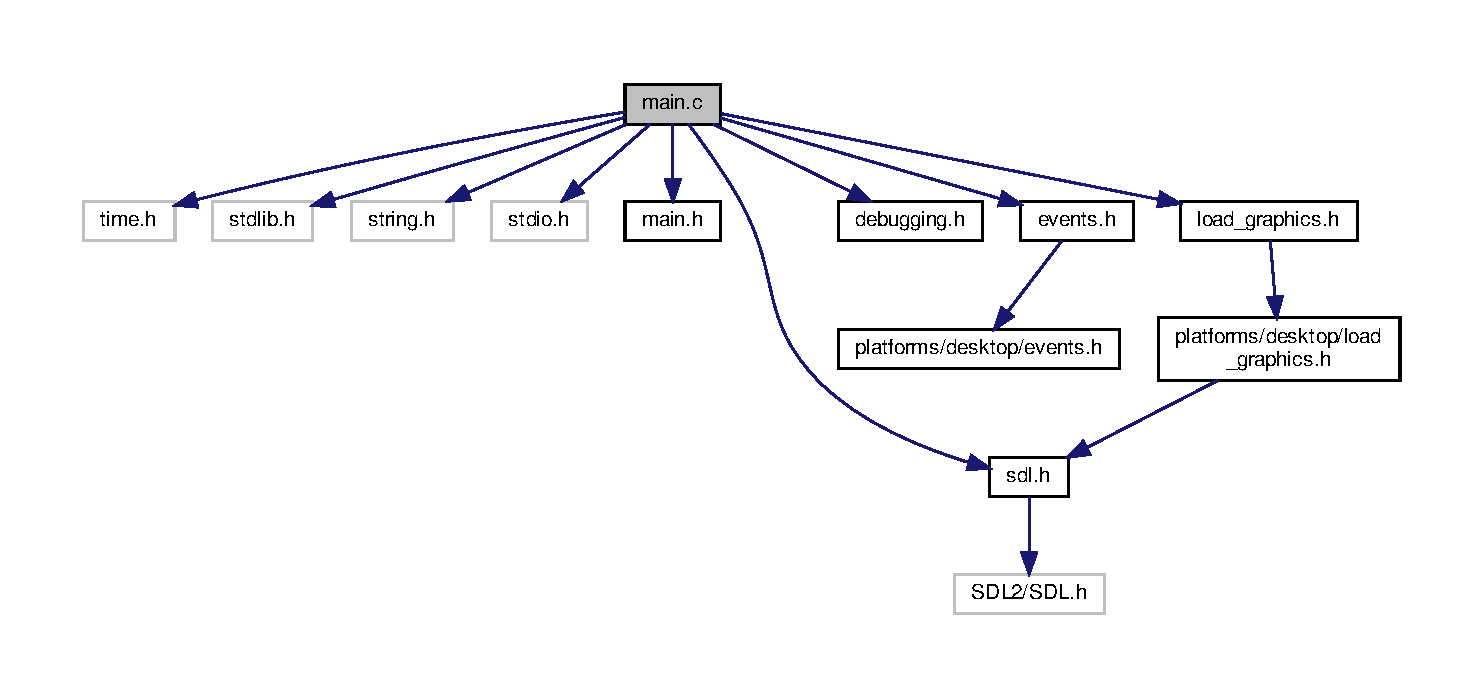
\includegraphics[width=350pt]{main_8c__incl}
\end{center}
\end{figure}
\subsection*{Classes}
\begin{DoxyCompactItemize}
\item 
struct \hyperlink{structttm}{ttm}
\begin{DoxyCompactList}\small\item\em structure for tetriminos \end{DoxyCompactList}\end{DoxyCompactItemize}
\subsection*{Macros}
\begin{DoxyCompactItemize}
\item 
\mbox{\Hypertarget{main_8c_aed89bd71aee8be823e8a20ec4e093c1e}\label{main_8c_aed89bd71aee8be823e8a20ec4e093c1e}} 
\#define {\bfseries H\+E\+I\+G\+HT}~18
\item 
\mbox{\Hypertarget{main_8c_a241aeeb764887ae5e3de58b98f04b16d}\label{main_8c_a241aeeb764887ae5e3de58b98f04b16d}} 
\#define {\bfseries W\+I\+D\+TH}~12
\item 
\mbox{\Hypertarget{main_8c_a5394435edf20efdffac70b5c362ade81}\label{main_8c_a5394435edf20efdffac70b5c362ade81}} 
\#define {\bfseries B\+L\+K\+\_\+\+S\+I\+ZE}~32
\item 
\mbox{\Hypertarget{main_8c_a6974d08a74da681b3957b2fead2608b8}\label{main_8c_a6974d08a74da681b3957b2fead2608b8}} 
\#define {\bfseries S\+C\+R\+E\+E\+N\+\_\+\+H\+E\+I\+G\+HT}~B\+L\+K\+\_\+\+S\+I\+ZE $\ast$ H\+E\+I\+G\+HT
\item 
\mbox{\Hypertarget{main_8c_a2cd109632a6dcccaa80b43561b1ab700}\label{main_8c_a2cd109632a6dcccaa80b43561b1ab700}} 
\#define {\bfseries S\+C\+R\+E\+E\+N\+\_\+\+W\+I\+D\+TH}~B\+L\+K\+\_\+\+S\+I\+ZE $\ast$ W\+I\+D\+TH
\item 
\mbox{\Hypertarget{main_8c_a316524eb48cf16cba5db0dd2e1c6a827}\label{main_8c_a316524eb48cf16cba5db0dd2e1c6a827}} 
\#define {\bfseries T\+T\+M\+\_\+\+W\+I\+D\+TH}~4
\end{DoxyCompactItemize}
\subsection*{Functions}
\begin{DoxyCompactItemize}
\item 
\mbox{\Hypertarget{main_8c_afc06c12631b3b00efa5659b921e9fdaa}\label{main_8c_afc06c12631b3b00efa5659b921e9fdaa}} 
int {\bfseries set\+Back\+Color} (S\+D\+L\+\_\+\+Renderer $\ast$renderer, S\+D\+L\+\_\+\+Color color)
\item 
int \hyperlink{main_8c_ada4dde753d303013ded20363eb1f9be9}{can\+Print} (char mat\mbox{[}T\+T\+M\+\_\+\+W\+I\+D\+TH\mbox{]}\mbox{[}T\+T\+M\+\_\+\+W\+I\+D\+TH\mbox{]}, int row, int col)
\begin{DoxyCompactList}\small\item\em Determines ability to print tetrimino. \end{DoxyCompactList}\item 
int \hyperlink{main_8c_a9c0090634c39398bd8865043616f6915}{rotate\+Cur} (void)
\begin{DoxyCompactList}\small\item\em rotate current tetrimino \end{DoxyCompactList}\item 
int \hyperlink{main_8c_a3a6ff3f3cf987dfe7ef29c8150d94dc5}{whole\+Line} (int row)
\begin{DoxyCompactList}\small\item\em determines if line is whole \end{DoxyCompactList}\item 
int \hyperlink{main_8c_acf4ebdb374829d8d913a822fcd73031f}{rand\+Ttm} (void)
\begin{DoxyCompactList}\small\item\em change current tetrimino to a random tetrimino \end{DoxyCompactList}\item 
int \hyperlink{main_8c_ae9692ec823f821130e4efaa40a72a2cb}{print\+Ttm} (char mat\mbox{[}T\+T\+M\+\_\+\+W\+I\+D\+TH\mbox{]}\mbox{[}T\+T\+M\+\_\+\+W\+I\+D\+TH\mbox{]}, int row, int col)
\begin{DoxyCompactList}\small\item\em put a tetrimino in the board \end{DoxyCompactList}\item 
\mbox{\Hypertarget{main_8c_aa6c6b91b693075c8ae01385351cdc971}\label{main_8c_aa6c6b91b693075c8ae01385351cdc971}} 
void \hyperlink{main_8c_aa6c6b91b693075c8ae01385351cdc971}{down\+Ttm} (void)
\begin{DoxyCompactList}\small\item\em down current tetrimino from 1 row \end{DoxyCompactList}\item 
\mbox{\Hypertarget{main_8c_a73c634b9e4f572e8c8a6843ab19640ca}\label{main_8c_a73c634b9e4f572e8c8a6843ab19640ca}} 
void \hyperlink{main_8c_a73c634b9e4f572e8c8a6843ab19640ca}{full\+Down\+Ttm} (void)
\begin{DoxyCompactList}\small\item\em down current tetrimino at the bottom \end{DoxyCompactList}\item 
void \hyperlink{main_8c_a3f1fb9940a8904e21137a65f45cb9436}{move\+Ttm} (int direction)
\begin{DoxyCompactList}\small\item\em move current tetrimino to left or right \end{DoxyCompactList}\item 
void \hyperlink{main_8c_a3d150ccfeb33959cda572f9cda9e6d80}{remove\+Line} (int row)
\begin{DoxyCompactList}\small\item\em Removes blocks from line and down the above ones. \end{DoxyCompactList}\item 
void \hyperlink{main_8c_ab59b086c41d506e55aa02729f9916be2}{refresh\+Screen} (void)
\begin{DoxyCompactList}\small\item\em refresh screen \end{DoxyCompactList}\item 
\mbox{\Hypertarget{main_8c_a27113921347a82199b52e4f2ee16985c}\label{main_8c_a27113921347a82199b52e4f2ee16985c}} 
void \hyperlink{main_8c_a27113921347a82199b52e4f2ee16985c}{game} (void)
\begin{DoxyCompactList}\small\item\em the place that contains game loop \end{DoxyCompactList}\item 
\mbox{\Hypertarget{main_8c_ac482f340f2b07e8a8e3432558beca16f}\label{main_8c_ac482f340f2b07e8a8e3432558beca16f}} 
int {\bfseries init} (S\+D\+L\+\_\+\+Window $\ast$window)
\item 
\mbox{\Hypertarget{main_8c_a0ddf1224851353fc92bfbff6f499fa97}\label{main_8c_a0ddf1224851353fc92bfbff6f499fa97}} 
int {\bfseries main} (int argc, char $\ast$argv\mbox{[}$\,$\mbox{]})
\end{DoxyCompactItemize}
\subsection*{Variables}
\begin{DoxyCompactItemize}
\item 
char {\bfseries I\+Ttm} \mbox{[}$\,$\mbox{]}\mbox{[}T\+T\+M\+\_\+\+W\+I\+D\+TH\mbox{]}
\item 
char {\bfseries L\+Ttm} \mbox{[}$\,$\mbox{]}\mbox{[}T\+T\+M\+\_\+\+W\+I\+D\+TH\mbox{]}
\item 
char {\bfseries J\+Ttm} \mbox{[}$\,$\mbox{]}\mbox{[}T\+T\+M\+\_\+\+W\+I\+D\+TH\mbox{]}
\item 
char {\bfseries T\+Ttm} \mbox{[}$\,$\mbox{]}\mbox{[}T\+T\+M\+\_\+\+W\+I\+D\+TH\mbox{]}
\item 
char {\bfseries O\+Ttm} \mbox{[}$\,$\mbox{]}\mbox{[}T\+T\+M\+\_\+\+W\+I\+D\+TH\mbox{]}
\item 
char {\bfseries Z\+Ttm} \mbox{[}$\,$\mbox{]}\mbox{[}T\+T\+M\+\_\+\+W\+I\+D\+TH\mbox{]}
\item 
char {\bfseries S\+Ttm} \mbox{[}$\,$\mbox{]}\mbox{[}T\+T\+M\+\_\+\+W\+I\+D\+TH\mbox{]}
\item 
\mbox{\Hypertarget{main_8c_ae18ac556fad863e56fdff8263c2b93f0}\label{main_8c_ae18ac556fad863e56fdff8263c2b93f0}} 
S\+D\+L\+\_\+\+Color {\bfseries white} = \{ 255, 255, 255, 255 \}
\item 
\mbox{\Hypertarget{main_8c_a0171f2945adf504f88fedaf624abfc6e}\label{main_8c_a0171f2945adf504f88fedaf624abfc6e}} 
S\+D\+L\+\_\+\+Color {\bfseries black} = \{ 0, 0, 0, 0 \}
\item 
\mbox{\Hypertarget{main_8c_af9dca46b01a2804b8730516485296199}\label{main_8c_af9dca46b01a2804b8730516485296199}} 
struct \hyperlink{structttm}{ttm} {\bfseries cur\+Ttm}
\item 
\mbox{\Hypertarget{main_8c_a27fdc41ce6ab40ec765e80ccbdbbee59}\label{main_8c_a27fdc41ce6ab40ec765e80ccbdbbee59}} 
char {\bfseries board} \mbox{[}H\+E\+I\+G\+HT\mbox{]}\mbox{[}W\+I\+D\+TH\mbox{]} = \{ 0 \}
\item 
\mbox{\Hypertarget{main_8c_ad8bbfd2bf84211ba3735476bf37a0826}\label{main_8c_ad8bbfd2bf84211ba3735476bf37a0826}} 
long {\bfseries score} = 0
\item 
\mbox{\Hypertarget{main_8c_a04de29e8773420834a86eb73e5ac07bf}\label{main_8c_a04de29e8773420834a86eb73e5ac07bf}} 
S\+D\+L\+\_\+\+Texture $\ast$ {\bfseries B\+LK}
\item 
\mbox{\Hypertarget{main_8c_a966da7a60c4ea3ba301e26ccc5efe452}\label{main_8c_a966da7a60c4ea3ba301e26ccc5efe452}} 
S\+D\+L\+\_\+\+Renderer $\ast$ {\bfseries renderer}
\end{DoxyCompactItemize}


\subsection{Detailed Description}
main part of the code 

\char`\"{}ttm\char`\"{} is an abbreviation for \char`\"{}tetrimino\char`\"{}. 

\subsection{Function Documentation}
\mbox{\Hypertarget{main_8c_ada4dde753d303013ded20363eb1f9be9}\label{main_8c_ada4dde753d303013ded20363eb1f9be9}} 
\index{main.\+c@{main.\+c}!can\+Print@{can\+Print}}
\index{can\+Print@{can\+Print}!main.\+c@{main.\+c}}
\subsubsection{\texorpdfstring{can\+Print()}{canPrint()}}
{\footnotesize\ttfamily int can\+Print (\begin{DoxyParamCaption}\item[{char}]{mat\mbox{[}\+T\+T\+M\+\_\+\+W\+I\+D\+T\+H\mbox{]}\mbox{[}\+T\+T\+M\+\_\+\+W\+I\+D\+T\+H\mbox{]},  }\item[{int}]{row,  }\item[{int}]{col }\end{DoxyParamCaption})}



Determines ability to print tetrimino. 


\begin{DoxyParams}[1]{Parameters}
 & {\em mat} & The matrix of the tetrimino \\
\hline
\mbox{\tt in}  & {\em row} & The row of the tetrimino \\
\hline
\mbox{\tt in}  & {\em col} & The column of the tetrimino\\
\hline
\end{DoxyParams}
\begin{DoxyReturn}{Returns}
1 if able to print, 0 otherwise. 
\end{DoxyReturn}
\mbox{\Hypertarget{main_8c_a3f1fb9940a8904e21137a65f45cb9436}\label{main_8c_a3f1fb9940a8904e21137a65f45cb9436}} 
\index{main.\+c@{main.\+c}!move\+Ttm@{move\+Ttm}}
\index{move\+Ttm@{move\+Ttm}!main.\+c@{main.\+c}}
\subsubsection{\texorpdfstring{move\+Ttm()}{moveTtm()}}
{\footnotesize\ttfamily void move\+Ttm (\begin{DoxyParamCaption}\item[{int}]{direction }\end{DoxyParamCaption})}



move current tetrimino to left or right 


\begin{DoxyParams}[1]{Parameters}
\mbox{\tt in}  & {\em direction} & The direction \\
\hline
\end{DoxyParams}
\mbox{\Hypertarget{main_8c_ae9692ec823f821130e4efaa40a72a2cb}\label{main_8c_ae9692ec823f821130e4efaa40a72a2cb}} 
\index{main.\+c@{main.\+c}!print\+Ttm@{print\+Ttm}}
\index{print\+Ttm@{print\+Ttm}!main.\+c@{main.\+c}}
\subsubsection{\texorpdfstring{print\+Ttm()}{printTtm()}}
{\footnotesize\ttfamily int print\+Ttm (\begin{DoxyParamCaption}\item[{char}]{mat\mbox{[}\+T\+T\+M\+\_\+\+W\+I\+D\+T\+H\mbox{]}\mbox{[}\+T\+T\+M\+\_\+\+W\+I\+D\+T\+H\mbox{]},  }\item[{int}]{row,  }\item[{int}]{col }\end{DoxyParamCaption})}



put a tetrimino in the board 


\begin{DoxyParams}[1]{Parameters}
\mbox{\tt in}  & {\em mat} & The matrix of the ttm \\
\hline
\mbox{\tt in}  & {\em row} & The row in board \\
\hline
\mbox{\tt in}  & {\em col} & The col in board\\
\hline
\end{DoxyParams}
\begin{DoxyReturn}{Returns}
1 if it\textquotesingle{}s not possible to print the ttm, 0 else 
\end{DoxyReturn}
\mbox{\Hypertarget{main_8c_acf4ebdb374829d8d913a822fcd73031f}\label{main_8c_acf4ebdb374829d8d913a822fcd73031f}} 
\index{main.\+c@{main.\+c}!rand\+Ttm@{rand\+Ttm}}
\index{rand\+Ttm@{rand\+Ttm}!main.\+c@{main.\+c}}
\subsubsection{\texorpdfstring{rand\+Ttm()}{randTtm()}}
{\footnotesize\ttfamily int rand\+Ttm (\begin{DoxyParamCaption}\item[{void}]{ }\end{DoxyParamCaption})}



change current tetrimino to a random tetrimino 

\begin{DoxyReturn}{Returns}
0 if current tetrimino successfully changed, 1 otherwise 
\end{DoxyReturn}
\mbox{\Hypertarget{main_8c_ab59b086c41d506e55aa02729f9916be2}\label{main_8c_ab59b086c41d506e55aa02729f9916be2}} 
\index{main.\+c@{main.\+c}!refresh\+Screen@{refresh\+Screen}}
\index{refresh\+Screen@{refresh\+Screen}!main.\+c@{main.\+c}}
\subsubsection{\texorpdfstring{refresh\+Screen()}{refreshScreen()}}
{\footnotesize\ttfamily void refresh\+Screen (\begin{DoxyParamCaption}\item[{void}]{ }\end{DoxyParamCaption})}



refresh screen 

remove everything from screen, refresh with content of {\itshape board} matrix, put current tetrimino at right place \mbox{\Hypertarget{main_8c_a3d150ccfeb33959cda572f9cda9e6d80}\label{main_8c_a3d150ccfeb33959cda572f9cda9e6d80}} 
\index{main.\+c@{main.\+c}!remove\+Line@{remove\+Line}}
\index{remove\+Line@{remove\+Line}!main.\+c@{main.\+c}}
\subsubsection{\texorpdfstring{remove\+Line()}{removeLine()}}
{\footnotesize\ttfamily void remove\+Line (\begin{DoxyParamCaption}\item[{int}]{row }\end{DoxyParamCaption})}



Removes blocks from line and down the above ones. 


\begin{DoxyParams}[1]{Parameters}
\mbox{\tt in}  & {\em row} & The line \\
\hline
\end{DoxyParams}
\mbox{\Hypertarget{main_8c_a9c0090634c39398bd8865043616f6915}\label{main_8c_a9c0090634c39398bd8865043616f6915}} 
\index{main.\+c@{main.\+c}!rotate\+Cur@{rotate\+Cur}}
\index{rotate\+Cur@{rotate\+Cur}!main.\+c@{main.\+c}}
\subsubsection{\texorpdfstring{rotate\+Cur()}{rotateCur()}}
{\footnotesize\ttfamily int rotate\+Cur (\begin{DoxyParamCaption}\item[{void}]{ }\end{DoxyParamCaption})}



rotate current tetrimino 

\begin{DoxyReturn}{Returns}
0 if current tetrimino successfully rotated, 1 otherwise 
\end{DoxyReturn}
\mbox{\Hypertarget{main_8c_a3a6ff3f3cf987dfe7ef29c8150d94dc5}\label{main_8c_a3a6ff3f3cf987dfe7ef29c8150d94dc5}} 
\index{main.\+c@{main.\+c}!whole\+Line@{whole\+Line}}
\index{whole\+Line@{whole\+Line}!main.\+c@{main.\+c}}
\subsubsection{\texorpdfstring{whole\+Line()}{wholeLine()}}
{\footnotesize\ttfamily int whole\+Line (\begin{DoxyParamCaption}\item[{int}]{row }\end{DoxyParamCaption})}



determines if line is whole 


\begin{DoxyParams}[1]{Parameters}
\mbox{\tt in}  & {\em row} & The line in the board\\
\hline
\end{DoxyParams}
\begin{DoxyReturn}{Returns}
1 if the line is whole, 0 otherwise 
\end{DoxyReturn}


\subsection{Variable Documentation}
\mbox{\Hypertarget{main_8c_a6e38d59b67e2f07ef7d581846d45eca1}\label{main_8c_a6e38d59b67e2f07ef7d581846d45eca1}} 
\index{main.\+c@{main.\+c}!I\+Ttm@{I\+Ttm}}
\index{I\+Ttm@{I\+Ttm}!main.\+c@{main.\+c}}
\subsubsection{\texorpdfstring{I\+Ttm}{ITtm}}
{\footnotesize\ttfamily char I\+Ttm\mbox{[}$\,$\mbox{]}\mbox{[}T\+T\+M\+\_\+\+W\+I\+D\+TH\mbox{]}}

{\bfseries Initial value\+:}
\begin{DoxyCode}
= \{
    \{ 0, 0, 1, 0 \},
    \{ 0, 0, 1, 0 \},
    \{ 0, 0, 1, 0 \},
    \{ 0, 0, 1, 0 \}
\}
\end{DoxyCode}
\mbox{\Hypertarget{main_8c_a92d0ffad508747d28c97c8007bed3c72}\label{main_8c_a92d0ffad508747d28c97c8007bed3c72}} 
\index{main.\+c@{main.\+c}!J\+Ttm@{J\+Ttm}}
\index{J\+Ttm@{J\+Ttm}!main.\+c@{main.\+c}}
\subsubsection{\texorpdfstring{J\+Ttm}{JTtm}}
{\footnotesize\ttfamily char J\+Ttm\mbox{[}$\,$\mbox{]}\mbox{[}T\+T\+M\+\_\+\+W\+I\+D\+TH\mbox{]}}

{\bfseries Initial value\+:}
\begin{DoxyCode}
= \{
    \{ 0, 0, 0, 0 \},
    \{ 0, 0, 1, 0 \},
    \{ 0, 0, 1, 0 \},
    \{ 0, 1, 1, 0 \}
\}
\end{DoxyCode}
\mbox{\Hypertarget{main_8c_ab78ffd76f6017442947eb891b33d9000}\label{main_8c_ab78ffd76f6017442947eb891b33d9000}} 
\index{main.\+c@{main.\+c}!L\+Ttm@{L\+Ttm}}
\index{L\+Ttm@{L\+Ttm}!main.\+c@{main.\+c}}
\subsubsection{\texorpdfstring{L\+Ttm}{LTtm}}
{\footnotesize\ttfamily char L\+Ttm\mbox{[}$\,$\mbox{]}\mbox{[}T\+T\+M\+\_\+\+W\+I\+D\+TH\mbox{]}}

{\bfseries Initial value\+:}
\begin{DoxyCode}
= \{
    \{ 0, 0, 0, 0 \},
    \{ 0, 1, 0, 0 \},
    \{ 0, 1, 0, 0 \},
    \{ 0, 1, 1, 0 \}
\}
\end{DoxyCode}
\mbox{\Hypertarget{main_8c_a644758571e4dd81bd24a2d795539aa8e}\label{main_8c_a644758571e4dd81bd24a2d795539aa8e}} 
\index{main.\+c@{main.\+c}!O\+Ttm@{O\+Ttm}}
\index{O\+Ttm@{O\+Ttm}!main.\+c@{main.\+c}}
\subsubsection{\texorpdfstring{O\+Ttm}{OTtm}}
{\footnotesize\ttfamily char O\+Ttm\mbox{[}$\,$\mbox{]}\mbox{[}T\+T\+M\+\_\+\+W\+I\+D\+TH\mbox{]}}

{\bfseries Initial value\+:}
\begin{DoxyCode}
= \{
    \{ 0, 0, 0, 0 \},
    \{ 0, 0, 0, 0 \},
    \{ 0, 1, 1, 0 \},
    \{ 0, 1, 1, 0 \}
\}
\end{DoxyCode}
\mbox{\Hypertarget{main_8c_a2080aa159a7afae0a3a2743aa111b8e0}\label{main_8c_a2080aa159a7afae0a3a2743aa111b8e0}} 
\index{main.\+c@{main.\+c}!S\+Ttm@{S\+Ttm}}
\index{S\+Ttm@{S\+Ttm}!main.\+c@{main.\+c}}
\subsubsection{\texorpdfstring{S\+Ttm}{STtm}}
{\footnotesize\ttfamily char S\+Ttm\mbox{[}$\,$\mbox{]}\mbox{[}T\+T\+M\+\_\+\+W\+I\+D\+TH\mbox{]}}

{\bfseries Initial value\+:}
\begin{DoxyCode}
= \{
    \{ 0, 0, 0, 0 \},
    \{ 0, 0, 0, 0 \},
    \{ 0, 1, 1, 0 \},
    \{ 1, 1, 0, 0 \}
\}
\end{DoxyCode}
\mbox{\Hypertarget{main_8c_ae14f1ce4231842d0848eb69d7dbc8a6e}\label{main_8c_ae14f1ce4231842d0848eb69d7dbc8a6e}} 
\index{main.\+c@{main.\+c}!T\+Ttm@{T\+Ttm}}
\index{T\+Ttm@{T\+Ttm}!main.\+c@{main.\+c}}
\subsubsection{\texorpdfstring{T\+Ttm}{TTtm}}
{\footnotesize\ttfamily char T\+Ttm\mbox{[}$\,$\mbox{]}\mbox{[}T\+T\+M\+\_\+\+W\+I\+D\+TH\mbox{]}}

{\bfseries Initial value\+:}
\begin{DoxyCode}
= \{
    \{ 0, 0, 0, 0 \},
    \{ 0, 1, 1, 1 \},
    \{ 0, 0, 1, 0 \},
    \{ 0, 0, 0, 0 \}
\}
\end{DoxyCode}
\mbox{\Hypertarget{main_8c_adaa3c91ca1c46e50586aab7f34760b60}\label{main_8c_adaa3c91ca1c46e50586aab7f34760b60}} 
\index{main.\+c@{main.\+c}!Z\+Ttm@{Z\+Ttm}}
\index{Z\+Ttm@{Z\+Ttm}!main.\+c@{main.\+c}}
\subsubsection{\texorpdfstring{Z\+Ttm}{ZTtm}}
{\footnotesize\ttfamily char Z\+Ttm\mbox{[}$\,$\mbox{]}\mbox{[}T\+T\+M\+\_\+\+W\+I\+D\+TH\mbox{]}}

{\bfseries Initial value\+:}
\begin{DoxyCode}
= \{
    \{ 0, 0, 0, 0 \},
    \{ 0, 0, 0, 0 \},
    \{ 0, 1, 1, 0 \},
    \{ 0, 0, 1, 1 \}
\}
\end{DoxyCode}

\hypertarget{desktop_2events_8c}{}\section{platforms/desktop/events.c File Reference}
\label{desktop_2events_8c}\index{platforms/desktop/events.\+c@{platforms/desktop/events.\+c}}
{\ttfamily \#include $<$stdlib.\+h$>$}\newline
{\ttfamily \#include \char`\"{}../../sdl.\+h\char`\"{}}\newline
{\ttfamily \#include \char`\"{}../../main.\+h\char`\"{}}\newline
Include dependency graph for events.\+c\+:
\nopagebreak
\begin{figure}[H]
\begin{center}
\leavevmode
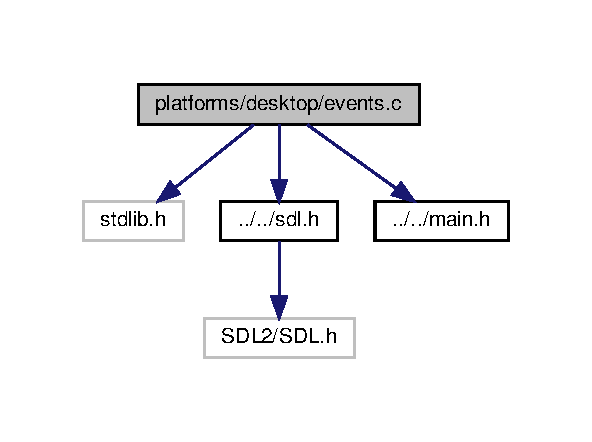
\includegraphics[width=284pt]{desktop_2events_8c__incl}
\end{center}
\end{figure}
\subsection*{Functions}
\begin{DoxyCompactItemize}
\item 
int \hyperlink{desktop_2events_8c_a27c6f8dbd1f752f7ed0eb59bf6fbf45a}{get\+Actions} (int $\ast$actions)
\begin{DoxyCompactList}\small\item\em Gets the actions of user. \end{DoxyCompactList}\end{DoxyCompactItemize}


\subsection{Function Documentation}
\mbox{\Hypertarget{desktop_2events_8c_a27c6f8dbd1f752f7ed0eb59bf6fbf45a}\label{desktop_2events_8c_a27c6f8dbd1f752f7ed0eb59bf6fbf45a}} 
\index{desktop/events.\+c@{desktop/events.\+c}!get\+Actions@{get\+Actions}}
\index{get\+Actions@{get\+Actions}!desktop/events.\+c@{desktop/events.\+c}}
\subsubsection{\texorpdfstring{get\+Actions()}{getActions()}}
{\footnotesize\ttfamily int get\+Actions (\begin{DoxyParamCaption}\item[{int $\ast$}]{actions }\end{DoxyParamCaption})}



Gets the actions of user. 

Actions of user are stored in {\itshape actions} global variable.


\begin{DoxyParams}{Parameters}
{\em actions} & The array of actions\\
\hline
\end{DoxyParams}
\begin{DoxyReturn}{Returns}
The number of actions 
\end{DoxyReturn}

\hypertarget{desktop_2load__graphics_8c}{}\section{platforms/desktop/load\+\_\+graphics.c File Reference}
\label{desktop_2load__graphics_8c}\index{platforms/desktop/load\+\_\+graphics.\+c@{platforms/desktop/load\+\_\+graphics.\+c}}
{\ttfamily \#include $<$stdlib.\+h$>$}\newline
{\ttfamily \#include \char`\"{}../../sdl.\+h\char`\"{}}\newline
Include dependency graph for load\+\_\+graphics.\+c\+:
\nopagebreak
\begin{figure}[H]
\begin{center}
\leavevmode
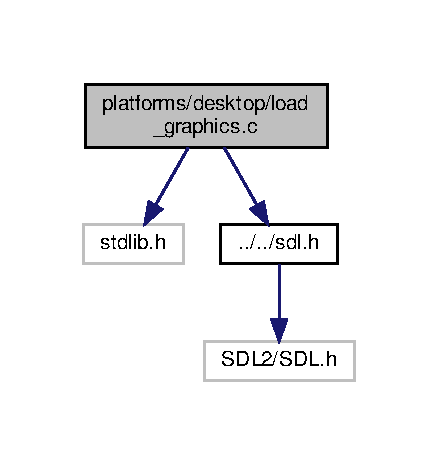
\includegraphics[width=210pt]{desktop_2load__graphics_8c__incl}
\end{center}
\end{figure}
\subsection*{Functions}
\begin{DoxyCompactItemize}
\item 
S\+D\+L\+\_\+\+Texture $\ast$ \hyperlink{desktop_2load__graphics_8c_a3dd89e1a3c52d876f71eddd894d9d0e7}{load\+Blk} (S\+D\+L\+\_\+\+Renderer $\ast$renderer)
\begin{DoxyCompactList}\small\item\em Gets block texture. \end{DoxyCompactList}\end{DoxyCompactItemize}
\subsection*{Variables}
\begin{DoxyCompactItemize}
\item 
\mbox{\Hypertarget{desktop_2load__graphics_8c_a87f875bbc08c891a30710c48b8406a99}\label{desktop_2load__graphics_8c_a87f875bbc08c891a30710c48b8406a99}} 
char $\ast$$\ast$ {\bfseries xpm\+Blk}
\end{DoxyCompactItemize}


\subsection{Function Documentation}
\mbox{\Hypertarget{desktop_2load__graphics_8c_a3dd89e1a3c52d876f71eddd894d9d0e7}\label{desktop_2load__graphics_8c_a3dd89e1a3c52d876f71eddd894d9d0e7}} 
\index{desktop/load\+\_\+graphics.\+c@{desktop/load\+\_\+graphics.\+c}!load\+Blk@{load\+Blk}}
\index{load\+Blk@{load\+Blk}!desktop/load\+\_\+graphics.\+c@{desktop/load\+\_\+graphics.\+c}}
\subsubsection{\texorpdfstring{load\+Blk()}{loadBlk()}}
{\footnotesize\ttfamily S\+D\+L\+\_\+\+Texture$\ast$ load\+Blk (\begin{DoxyParamCaption}\item[{S\+D\+L\+\_\+\+Renderer $\ast$}]{renderer }\end{DoxyParamCaption})}



Gets block texture. 


\begin{DoxyParams}{Parameters}
{\em renderer} & The S\+DL renderer\\
\hline
\end{DoxyParams}
\begin{DoxyReturn}{Returns}
S\+DL texture of the red block 
\end{DoxyReturn}

%--- End generated contents ---

% Index
\backmatter
\newpage
\phantomsection
\clearemptydoublepage
\addcontentsline{toc}{chapter}{Index}
\printindex

\end{document}
